\documentclass[12pt]{article}
\usepackage[paper=a4paper,left=25mm,right=25mm,top=25mm,bottom=25mm]{geometry}
\usepackage[english]{babel}
\usepackage[utf8]{inputenc}
\usepackage[pdftex]{graphicx}
\usepackage{color}
\usepackage{amssymb}
\usepackage{amsthm}
\usepackage{hyperref}
\usepackage{enumitem}
\usepackage{pdfpages}
\usepackage{hyperref}
\usepackage{subcaption}


\linespread{1.25}

\begin{document}
\begin{titlepage}
% 
\includegraphics[height=20mm]{images/uzh_logo}\\

\begin{flushleft}

\vspace{2cm}

{\Large Introduction to Artificial Intelligence\\Exercise Sheet 2}\\

\vspace{4cm}

\textbf{Laurin van den Bergh, 16-744-401\\Yufeng Xiao, 19-763-663\\Nora Beringer, 19-734-227}\\

\vspace{2cm}

Universität Zürich\\
Institut für Informatik

\vfill Due: March 9, 2022

\vspace{3cm}


\end{flushleft}
\end{titlepage}

\newpage

\section*{Exercise 2.1}
farmer = f, wolf = w, goat = g, cabbage = c \newline \newline
States:  S = $\langle f, w, g, c \rangle, f, c, g, w \in \{ L, R \}$ ; We can ignore the boat as we assume the boat is always where the farmer's at.\newline
Initial state: $\langle L, L, L, L \rangle$ \newline
Goal states: $\langle$ R, R, R, R $\rangle$ ; we find that four states are sink states and therefore don't offer a valid goal states in order to solve the riddle. These are: $\langle L, R, \cdot , R \rangle$, $\langle L, \cdot , R, R \rangle$, $\langle R, \cdot, L, L \rangle$, $\langle R, L, \cdot, L \rangle$ where $\cdot \in \{ L, R \}.$ \\
Actions: $\{ move$\_$c, move$\_$g, move$\_$w\}$ ;we assume moving each individual item also moves the farmer.  \newline
Transition model: T: S x A $\to$ S $\cup \{\perp \}$ \\ \\ 
Note: Farmer is the first position, wolf 2nd, goat 3rd and cabbage 4th \\ \\\hspace*{25mm}%
$\langle L,L,L,L \rangle$ \\ \hspace*{35mm}%
$ \downarrow$ \\ \hspace*{25mm}%
$\langle R,L,R,L \rangle$ \\ \hspace*{35mm}%
$\downarrow$ \\ \hspace*{25mm}%
$\langle L,L,R,L \rangle$ \\ \hspace*{10mm}%
$\swarrow$ \hspace*{40mm}%
$\searrow$ \\
$\langle R,R,R,L \rangle$ \hspace*{25mm}%
$\langle R,L,R,R \rangle$ \\ \hspace*{10mm}%
$\searrow$ \hspace*{40mm}%
$\swarrow \\ \\ \langle L,R,L,L \rangle$ \hspace*{25mm}%
$\langle L,L,L,R \rangle$ \\ \hspace*{35mm}%
$\downarrow$ \\ \hspace*{25mm}%
$\langle R,R,L,R \rangle$ \\ \hspace*{35mm}%
$\downarrow$ \\ \\ \hspace*{25mm}%
$\langle L,R,L,R \rangle$ \\ \hspace*{35mm}%
$\downarrow$ \\ \hspace*{25mm}%
$\langle R,R,R,R \rangle$ \newpage


\section*{Exercise 2.2}

\begin{enumerate}
    \item[a)] Incorrect. If the algorithm doesn't take into account of states already visited, then it could visit each state an infinite number of times. 
    \item[b)] False, it isn't complete but it is useful as it uses less memory, implements an acyclic state space and works faster then BFS.  
    \item[c)] True, because BFS with uniform cost is complete and optimal.
    \item[d)] In uniform-cost search, goal test on the node is performed when it is selcted for expansion. Otherwise the first node generated could be a sub-optimal path. Hence with early goal testing the search is cost optimal.
    \item[e)] Correct as it combines the benefits of BFS and DFS and one can limit the depth.\newline
\end{enumerate}

\section*{Exercise 2.3}

% \begin{figure}[h!]
%     \centering
%     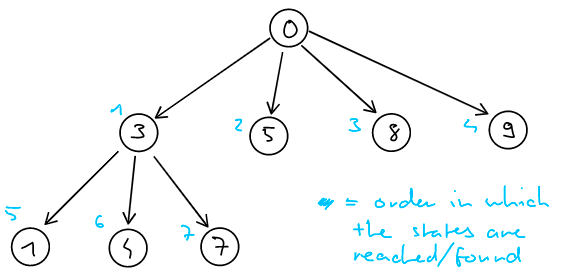
\includegraphics[width=.7\textwidth]{sheet02_3a.png}
% \end{figure}

\begin{figure}[h!]
    \begin{subfigure}{0.5\textwidth}
        \centering
        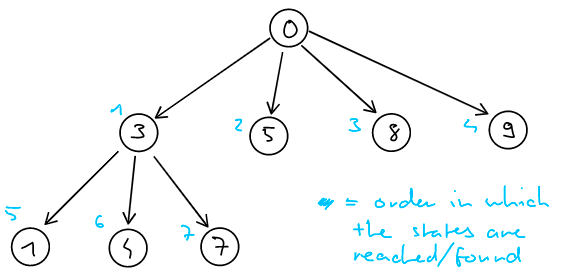
\includegraphics[width=\textwidth]{sheet02_3a.png}
        \caption{}
    \end{subfigure}
    \begin{subfigure}{0.5\textwidth}
        \centering
        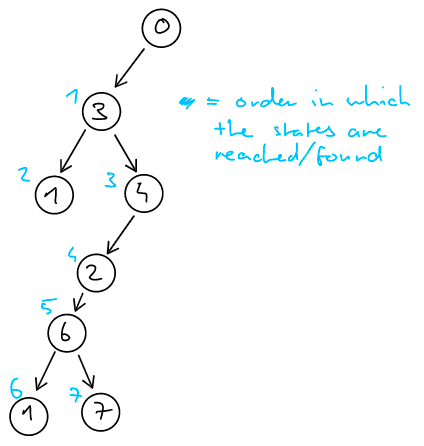
\includegraphics[width=\textwidth]{sheet02_3b.png}
        \caption{}
    \end{subfigure}
    \caption{(a) Shows the search tree of the breadth first search algorithm, (b) shows the search tree of the depth first search algorithm. The numbers in blue denote the order in which the states are explored.}
\end{figure}





\end{document}